\documentclass[tikz,border=2pt]{standalone}
\usepackage{amsmath,amssymb}
\usepackage{tikz}

\begin{document}
% A ⊂ B (proper): A lies inside B and B has at least one element outside A.
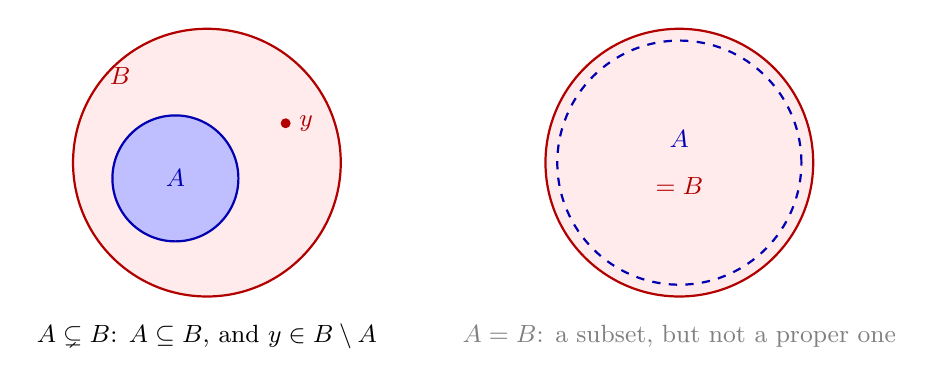
\begin{tikzpicture}[every node/.style={font=\small}]
	\draw[thick, red!70!black, fill=red!8] (0,0) circle (1.7);
	\draw[thick, blue!70!black, fill=blue!25] (-0.4,-0.2) circle (0.8);
	\node[blue!70!black] at (-0.4,-0.2) {$A$};
	\node[red!70!black] at (-1.1,1.1) {$B$};
	\fill[red!70!black] (1.0,0.5) circle (1.8pt);
	\node[red!70!black, right] at (1.05,0.5) {$y$};
	\node at (0,-2.2) {$A\subsetneq B$: $A\subseteq B$, and $y\in B\setminus A$};
	\begin{scope}[xshift=6cm]
		\draw[thick, red!70!black, fill=red!8] (0,0) circle (1.7);
		\draw[thick, blue!70!black, dashed] (0,0) circle (1.55);
		\node[blue!70!black] at (0,0.3) {$A$};
		\node[red!70!black] at (0,-0.3) {$=B$};
		\node[gray] at (0,-2.2) {$A=B$: a subset, but not a proper one};
	\end{scope}
\end{tikzpicture}
\end{document}
